Diagramas de parâmetros são usados para descrever relacionamentos entre propriedades requeridas pelos sistema.

\subsubsection{Estrutura dos diagramas de parâmetros}

Os diagramas são construídos por blocos "base" e por blocos de restrição(\textit{constraints}), cada umas dessas restrições é uma equação matemática que precisa ser parametrizada.

Os blocos de restrição podem ser vinculados a constantes ou a outros blocos de restrição. Ou seja, uma restrição de um bloco pode ser o resultado dos parâmetros e restrições de outro bloco, o que permite uma visualização hierárquica das operações que precisam ser feitas.

Os Blocos são construídos por 3 partes, os parâmetros em sí:

\begin{itemize}
  \item \textbf{Nome:} Nome da restrição
  \item \textbf{Restrições:} Equações matemáticas, ou restrições vindas de outros blocos
  \item \textbf{Parâmetros:} Parâmetros a serem levados em conta nas equações 
\end{itemize}



\begin{figure}[h]
\centering
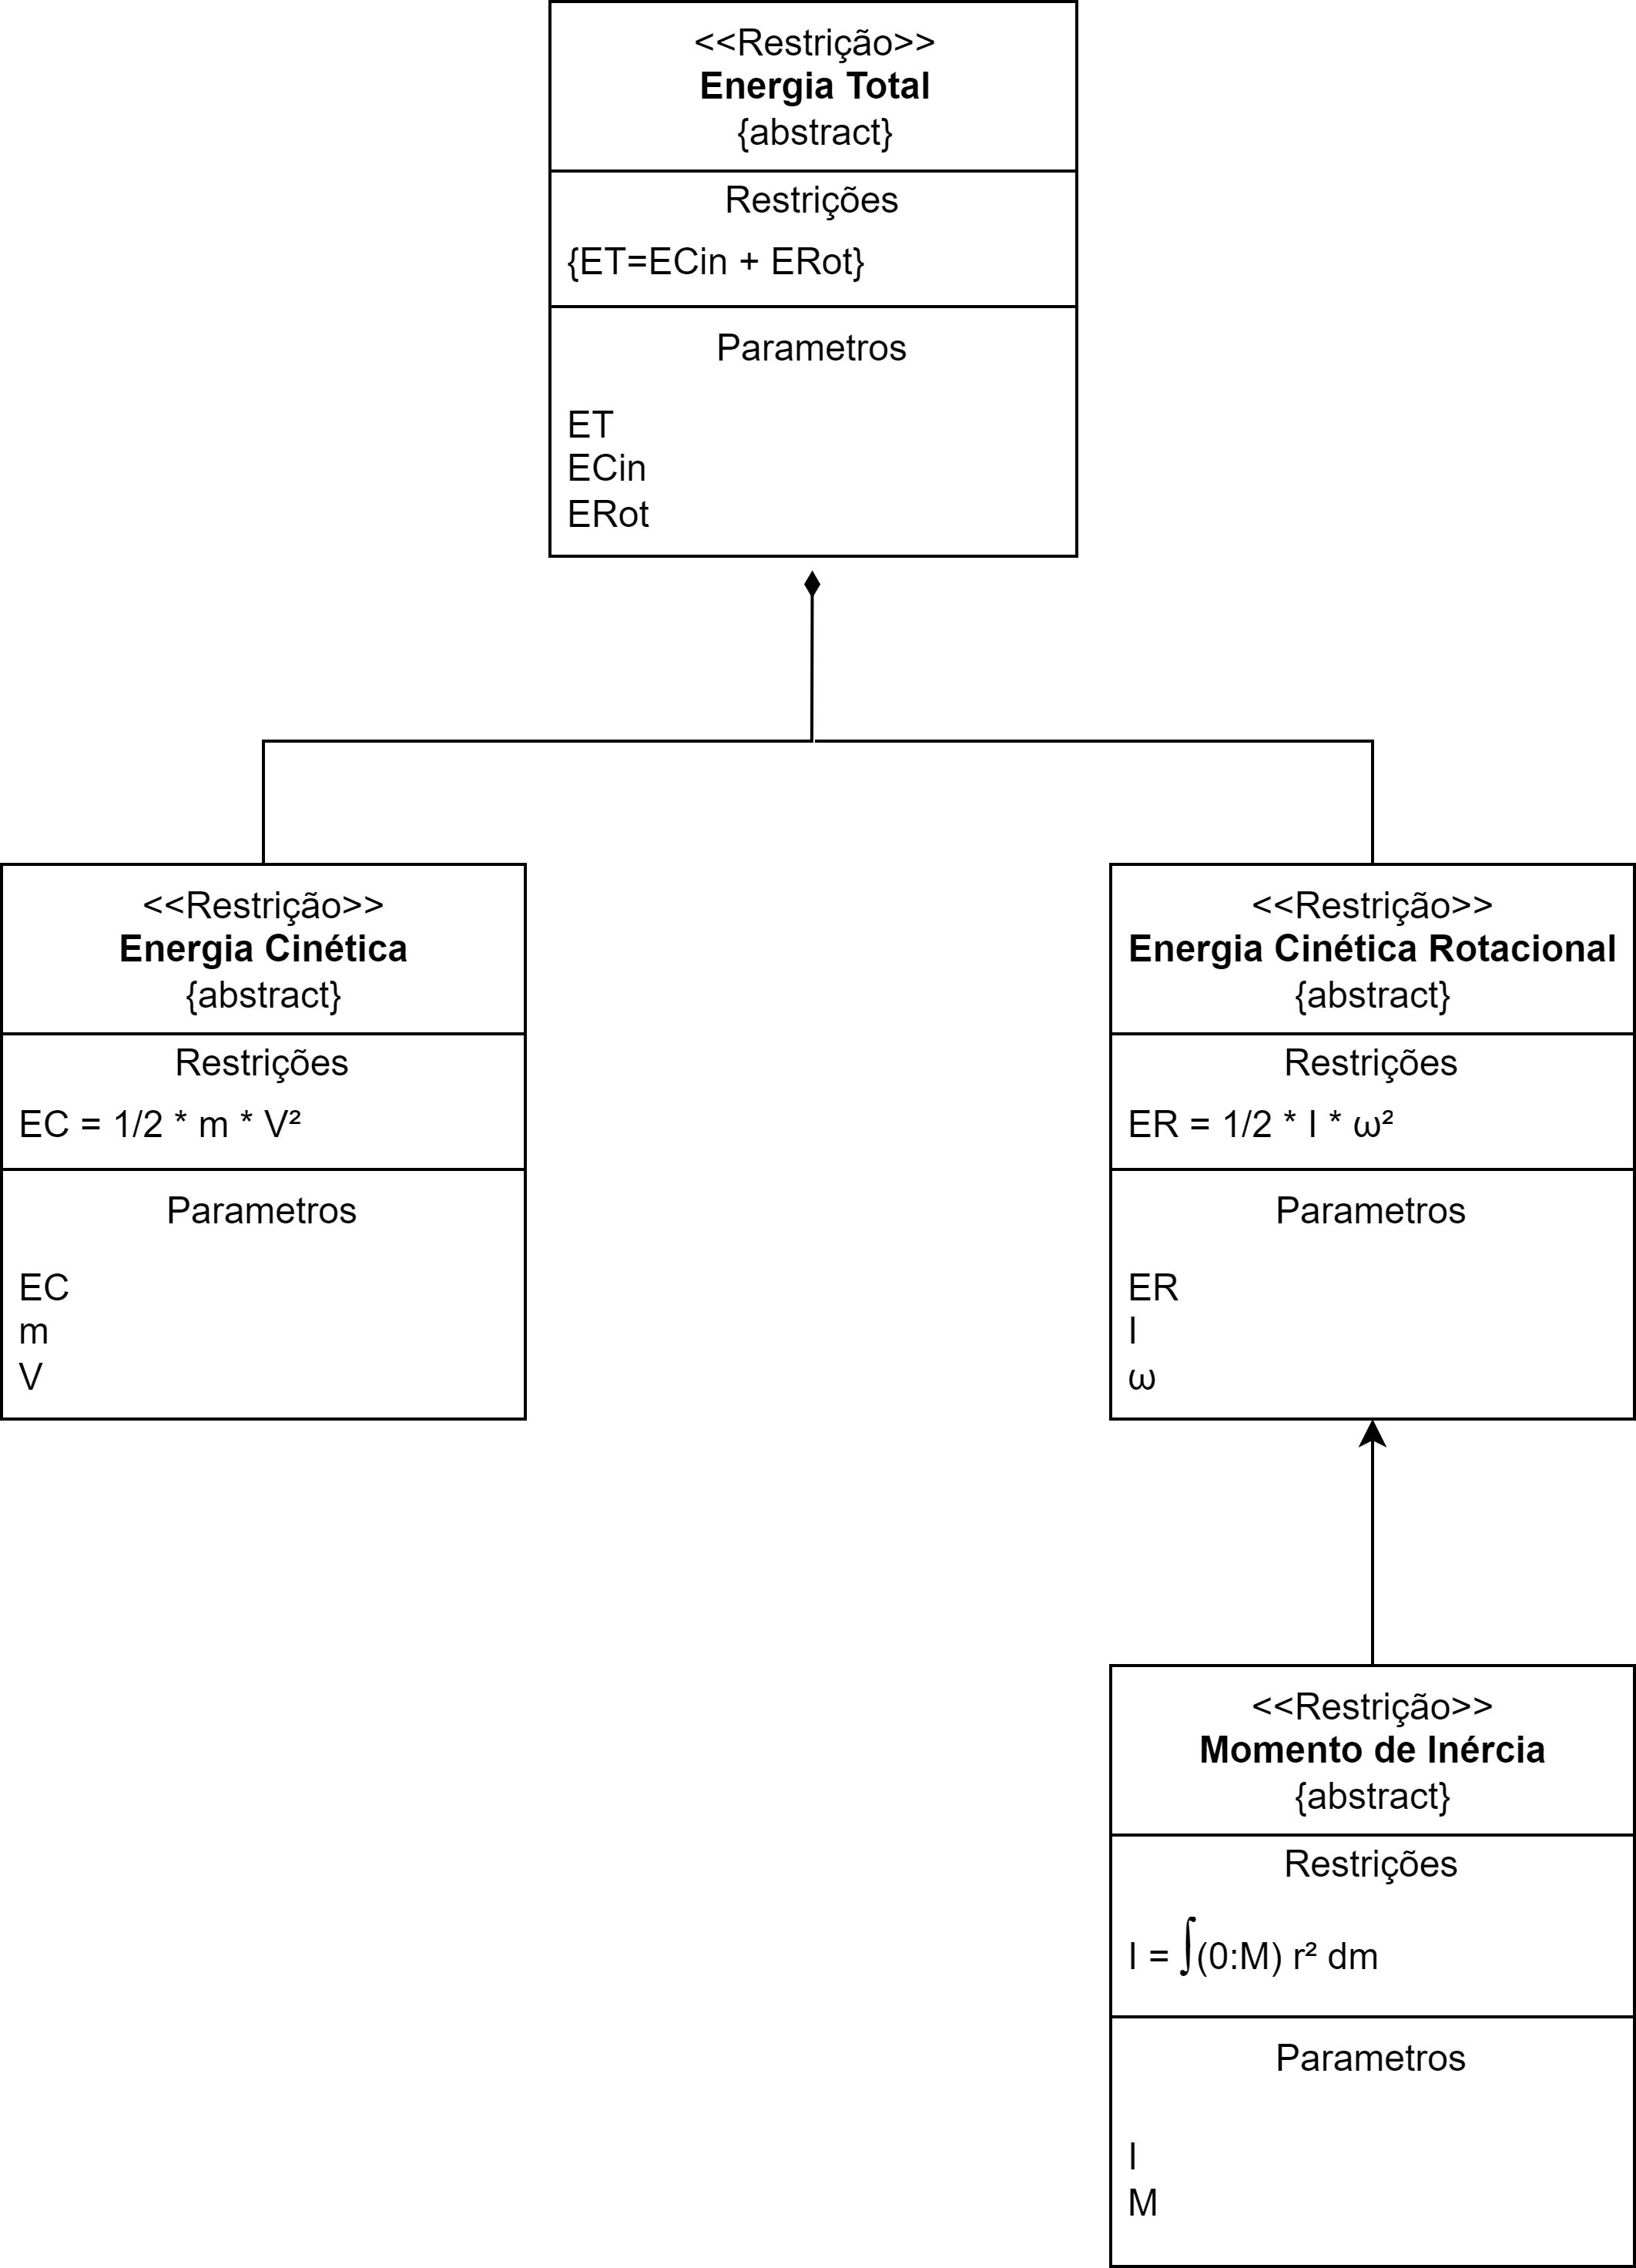
\includegraphics[width=\textwidth/2,height=\textheight,keepaspectratio]{figures/diagrama de parametros.png}
\caption{Diagrama de parâmetros}
\label{fig:parameter_diagram}
\end{figure}